%TC:group tabular 1 1
\subsection{Function calls}

\begin{figure}[H]
  \centering
  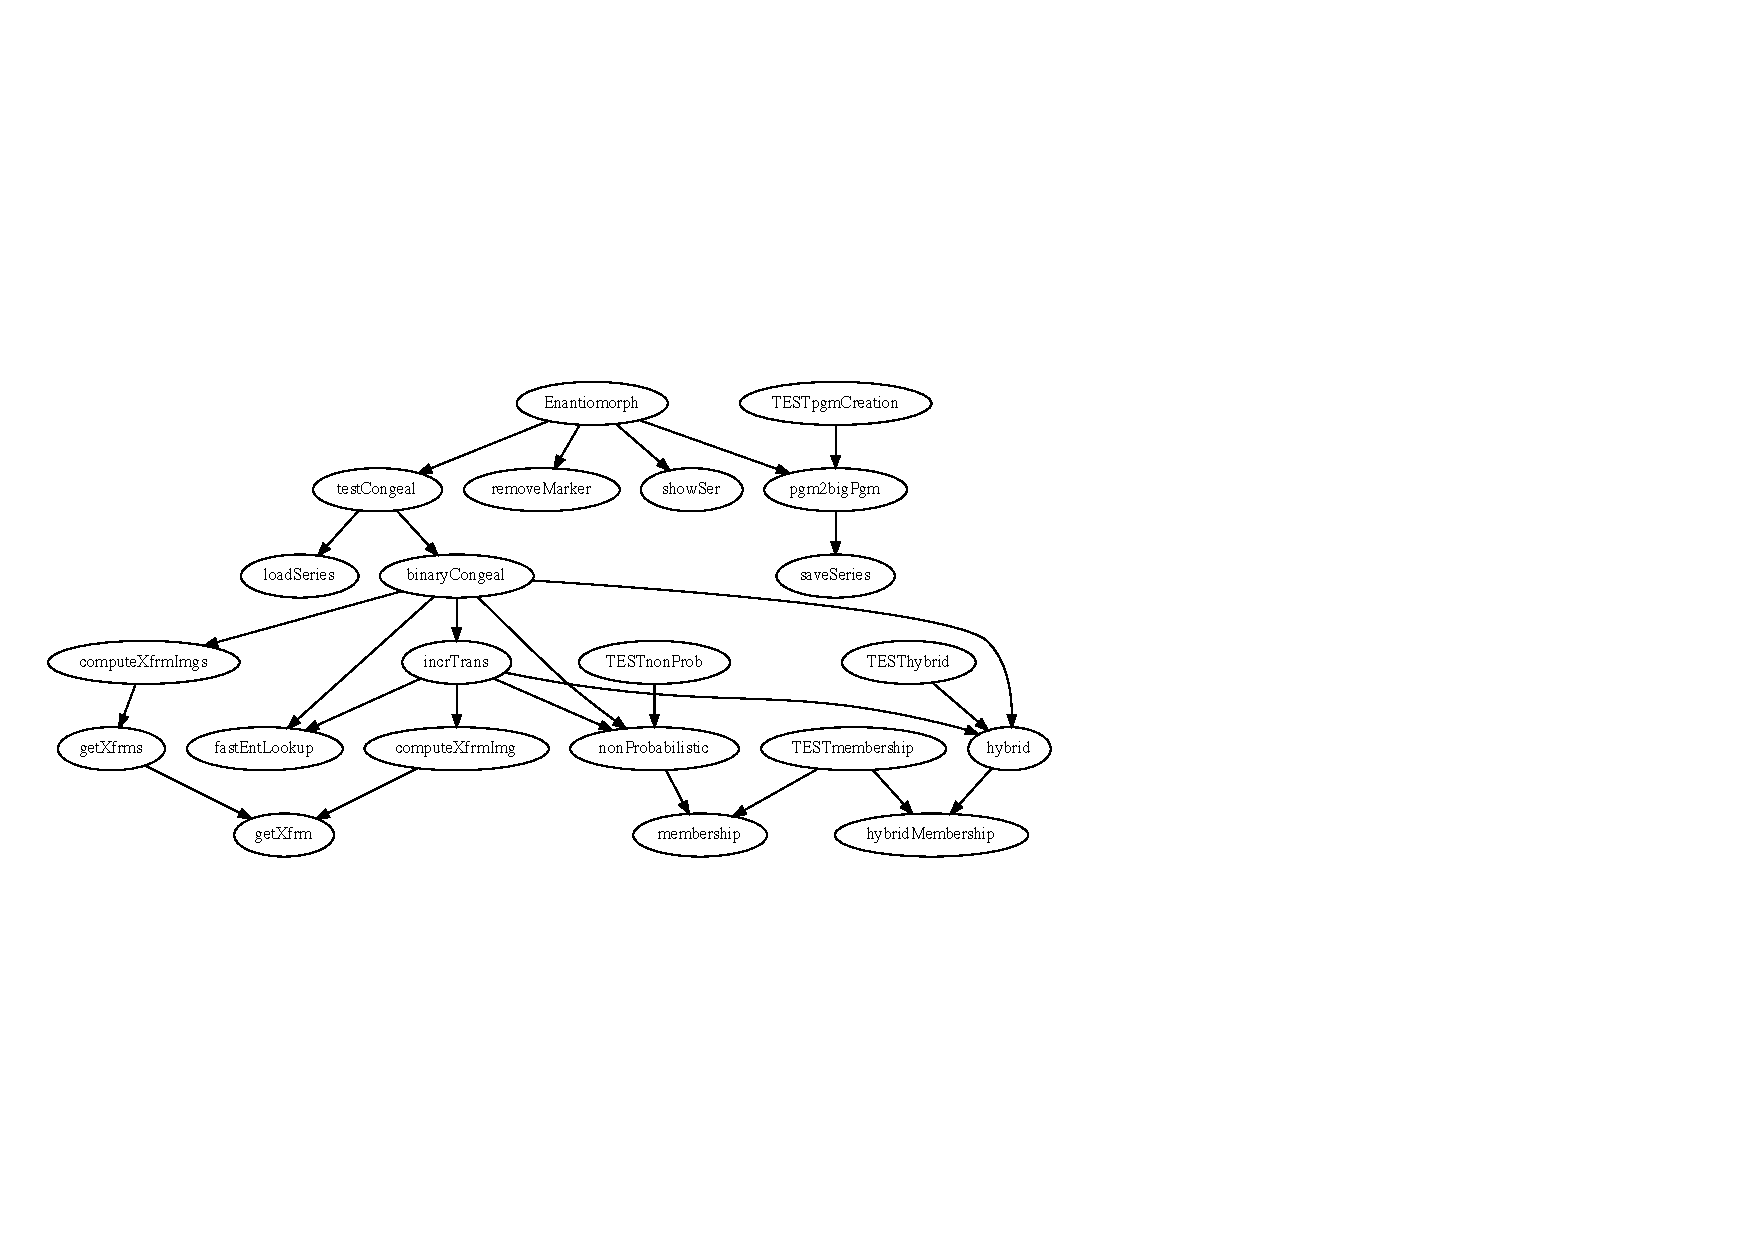
\includegraphics[width=\textwidth,clip,trim=0mm 50mm 110mm 50mm]{Chapter2/software-img/function_call_1.pdf}
  \caption{Function calls through the application.}
  \label{fig:data-flow}
\end{figure}

Figure \ref{fig:data-flow} shows which Function/Script calls which through the application, all the way up to \texttt{Enantiomorph}, the \acrshort{GUI}. This diagram shows the integration of new, modified and existing functions/scripts in the code-base, as listed in Appendix \ref{appendix:code}.

Diagrams such as this were helpful especially at the beginning of the project, due to working with an existing code-base. It was advantageous to see which functions were directly being called, and where the new functions for fuzzy entropy and membership would fit in.

\subsection{Testing}

Prior to the project beginning, it was outlined that this project would follow a \acrfull{TDD} practice. In \acrshort{TDD}, the Developer first writes a test, which will fail due to the lack of corresponding functionality. They would then go on to implement the functionality desired by the test. Finally, any refactoring of the initial test and/or code would take place.

However due to the nature of the project, it became increasingly more difficult to follow given the research which had to be undertaken alongside development. This led to a change from \acrshort{TDD} to Retrospective Testing, all tests would be written post-functional-implementation. This is a more traditional approach to testing, and still catches the same errors which might occur during \acrshort{TDD}.

\subsubsection{Unit Tests}

Unit Tests were completed using MATLAB's Unit Testing Framework \cite{testing}, which covers all the ways in which you can program in MATLAB:

\begin{itemize}
  \item Script-Based Unit Tests
  \item Function-Based Unit Tests
  \item Class-Based Unit Tests
  \end{itemize}

The majority of my work in MATLAB was function-based, so this was the style followed for unit tests. As Figure \ref{fig:unit-test-results} demonstrates, all Unit tests passed.

\begin{figure}[H]
  \centering
  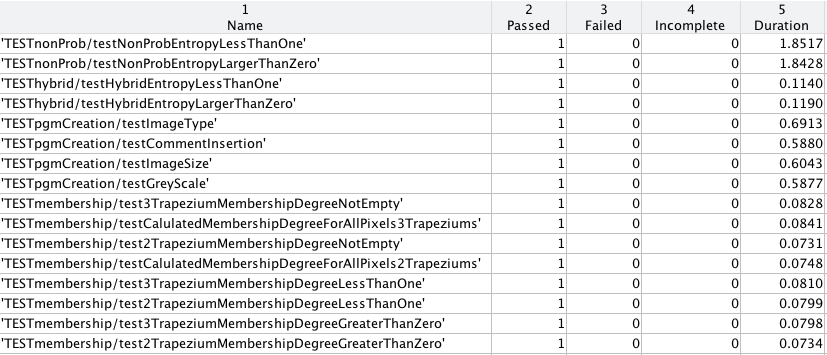
\includegraphics[width=\textwidth]{Chapter2/software-img/test-results.png}
  \caption{Results from MATLAB Unit Tests.}
  \label{fig:unit-test-results}
\end{figure}

\subsubsection{Acceptance Tests}

Acceptance tests are when each `requirement' is assessed in turn to assure its completion. In this project, as there was no firm requirements at the beginning of the process, the User Stories which were derived over the project duration will be assessed against. In \acrfull{XP}, a User Story is not considered to be complete until the time in which it passes its acceptance test, as stating on the \acrshort{XP} website \cite{Acceptance_Tests}.

Table \ref{table:acceptance} outlines the results from the Acceptance Tests run. The left-most column \say{User Story Reference} aligns with Table \ref{table:User Stories}, where more detail on each Story can be found.

\begin{center}
  \small
  \begin{longtable}{| p{2cm} | p{6cm} | p{2cm}  | p{1.5cm} |}
    \hline
      \textbf{User Story Reference} & \textbf{Expected Outcome} & \textbf{Actual \newline Outcome} & \textbf{Pass/Fail} \\ \hline \endhead
      1 & Image is loaded into the system & As expected & Pass \\ \hline
      2 & Membership array is passed out of the membership function and is usable in other functions & As expected & Pass \\ \hline
      3 & Images are aligned using Non-Probabilistic entropy and the output \& entropy outputs are realistic & As expected & Pass \\ \hline
      4 & Images are aligned using the metric the user has selected when running the function & As expected & Pass \\ \hline
      6 & The number of iterations is run as specified by the User, then function stops & As expected & Pass \\ \hline
      8 & Images are aligned using Shannon entropy and the output \& entropy outputs are realistic & As expected & Pass \\ \hline
      9 & Image(s) selected to be loaded into the GUI is displayed & As expected & Pass \\ \hline
      12 & Image box where input image appears goes blank after Clear button is selected & As expected & Pass \\ \hline
      13 & Images are aligned using Hybrid entropy and the output \& entropy outputs are realistic & As expected & Pass \\ \hline
      14 & Images are aligned using the chosen alignment metric & As expected & Pass \\ \hline
      15 & The number of iterations is run as specified by the User, then function stops & As expected & Pass \\ \hline
      16 & When an input image is loaded in, Metadata is displayed in the GUI about the image & As expected & Pass \\ \hline
      17 & After \Gls{Congealing}, the user can press the \say{See all Mean images} button and a new Figure displays the mean image after each iteration & As expected & Pass \\ \hline
      18 & After \Gls{Congealing}, the user can press the \say{See Adjusted Inputs} button and a new Figure displays the adjusted input images after the final iteration  & As expected & Pass \\ \hline
      21 & Image box where output image appears goes blank after Clear button is selected along with all other fields & As expected & Pass \\ \hline
      22 & Image is displayed larger in a new Figure & As expected & Pass \\ \hline
      23 & Save file dialog appears with a sensible name suggested (i.e. final image - alignment-chosen - number of iterations) & As expected & Pass \\ \hline
      24 & When \say{Entropy details} button is selected, a new Figure appears with a graph showing entropy decrease. Final Entropy \& time taken also displays in the main GUI & As expected & Pass \\ \hline
      25 & Egg-timer appears when \Gls{Congealing} Algorithm is running & As expected & Pass \\ \hline
      \caption{Acceptance Test results}
      \label{table:acceptance}
  \end{longtable}
\end{center}
